\chapter{Deployment}

L'applicazione è strutturata mediante i seguenti container:

\begin{itemize}
    \item Frontend Service: container che serve il Frontend sotto forma di Single Page Application.

    \item Messages Service e relativo Db: servizio responsabile della gestione dei messaggi testuali dell'applicazione (invio, ricezione, ecc...).

    \item Monitoring Service e relativo Db: servizio responsabile del monitoraggio dello stato di tutti i microservizi.

    \item Notifications Service e relativo Db: servizio responsabile delle notifiche degli utenti. Inoltre, detiene l'online status degli utenti del sistema.

    \item Piperchat Service e relativo Db: servizio responsabile della gestione dei Server e dei Canali dell'applicazione (creazione, modifica, partecipanti, ecc...).

    \item Users Service e relativo Db: servizio responsabile della gestione degli utenti dell'applicazione (login, registrazione, amicizie, ecc...).

    \item WebRTC Service e relativo Db: servizio responsabile della gestione delle chiamate infra-utenti e dei canali multimediali.

    \item Broker: container che ospita un server di \emph{RabbitMQ} per permettere lo scambio di messaggi all'interno del sistema

    \item Coturn: container che ospita il server \emph{TURN} (\url{https://github.com/coturn/coturn})

    \item Gateway: container che ospita l'\emph{API Gateway} realizzato con \emph{Traefik}. 

    \item Inspector: container di \emph{utility} per debuggare e/o ispezionare i servizi dall'interno della rete.
\end{itemize}

Per ogni microservizio quindi, viene effettuato il deploy di due diversi container, uno per il Webserver, mentre l'altro per il relativo database non relazionale.

Ogni microservizio possiede le seguenti reti docker:

\begin{itemize}
    \item Frontend: Per ricevere le richieste dal frontend tramite il Gateway.

    \item Backend: Per comunicare con gli altri microservizi (nel nostro caso tramite message broker).

    \item Microservicename-network: Rete interna del microservizio, utile alla comunicazione con il proprio database.
\end{itemize}

%
%
%
\section{Microservice deploy}

Per ogni microservizio è stato scritto un file \texttt{Docker Compose}.

Esempio di Docker compose relativo al singolo microservizio:

\begin{verbatim}
services:
  piperchat-service:
    image: piperchat
    command: [
        'npm', 
        'run', 
        '--workspace', 
        './services/piperchat', 
        'start'
    ]
    expose:
      - '${PIPERCHAT_SERVICE_PORT}'
    depends_on:
      db-piperchat-service:
        condition: service_healthy
      broker:
        condition: service_healthy
    networks:
      piperchat-network:
      backend:
        aliases:
          - ${PIPERCHAT_SERVICE_NAME}
      frontend:
    environment:
      - 'PORT=${PIPERCHAT_SERVICE_PORT}'
      - 'AMQP_URI=${BROKER_URI}'
      - 'MONGO_URI=
      mongodb://db-piperchat-service:27017/piperchat'
    labels:
      - |
        traefik.http.routers.piperchat-service.rule=
        (Method(`GET`, `POST`) 
            && Path(`/servers`)) ||
        (Method(`GET`, `PUT`, `DELETE`) 
            && Path(`/servers/{serverId:[^/]+}`)) ||
        (Method(`GET`, `POST`, `DELETE`) 
            && Path(`/servers/{serverId:[^/]+}/participants`)) ||
        (Method(`DELETE`) 
            && Path(`/servers/{serverId:[^/]+}/participants/{userId:[^/]+}`)) ||
        (Method(`GET`, `POST`) 
            && Path(`/servers/{serverId:[^/]+}/channels`)) ||
        (Method(`GET`, `PUT`, `DELETE`) 
            && Path(`/servers/{serverId:[^/]+}/channels/{channelId:[^/]+}`))

  db-piperchat-service:
    image: mongo
    expose:
      - '27017'
    volumes:
      - './.docker/db-piperchat:/data/db'
    healthcheck:
      test: |
        host=`hostname --ip-address || echo '127.0.0.1'`;
        mongo --quiet $${host}/test --eval 
        'quit(db.runCommand({ ping: 1 }).ok ? 0 : 2)' && echo 0 || echo 1
    networks:
      - piperchat-network

networks:
  piperchat-network:

\end{verbatim}

%
%
%
\section{Architecture deploy}

Avendo realizzato per ogni microservizio un apposito file  di \texttt{Docker Compose}, è stato utilizzato uno script bash per automatizzare l'unione di quest'ultimi ed eseguire il deploy dell'intera architettura.

Questo script si trova nella cartella root del progetto e si chiama \texttt{./deploy.sh}

Di seguito ne viene riportato un estratto:

\begin{verbatim}
docker compose \
    --project-name piperchat \
    --project-directory . \
    --env-file ./.env \
    -f ./services/broker/docker-compose.yaml \
    -f ./services/frontend/docker-compose.yaml \
    -f ./services/gateway/docker-compose.yaml \
    ...
    up
\end{verbatim}

\begin{figure}[htbp]
    \centering
    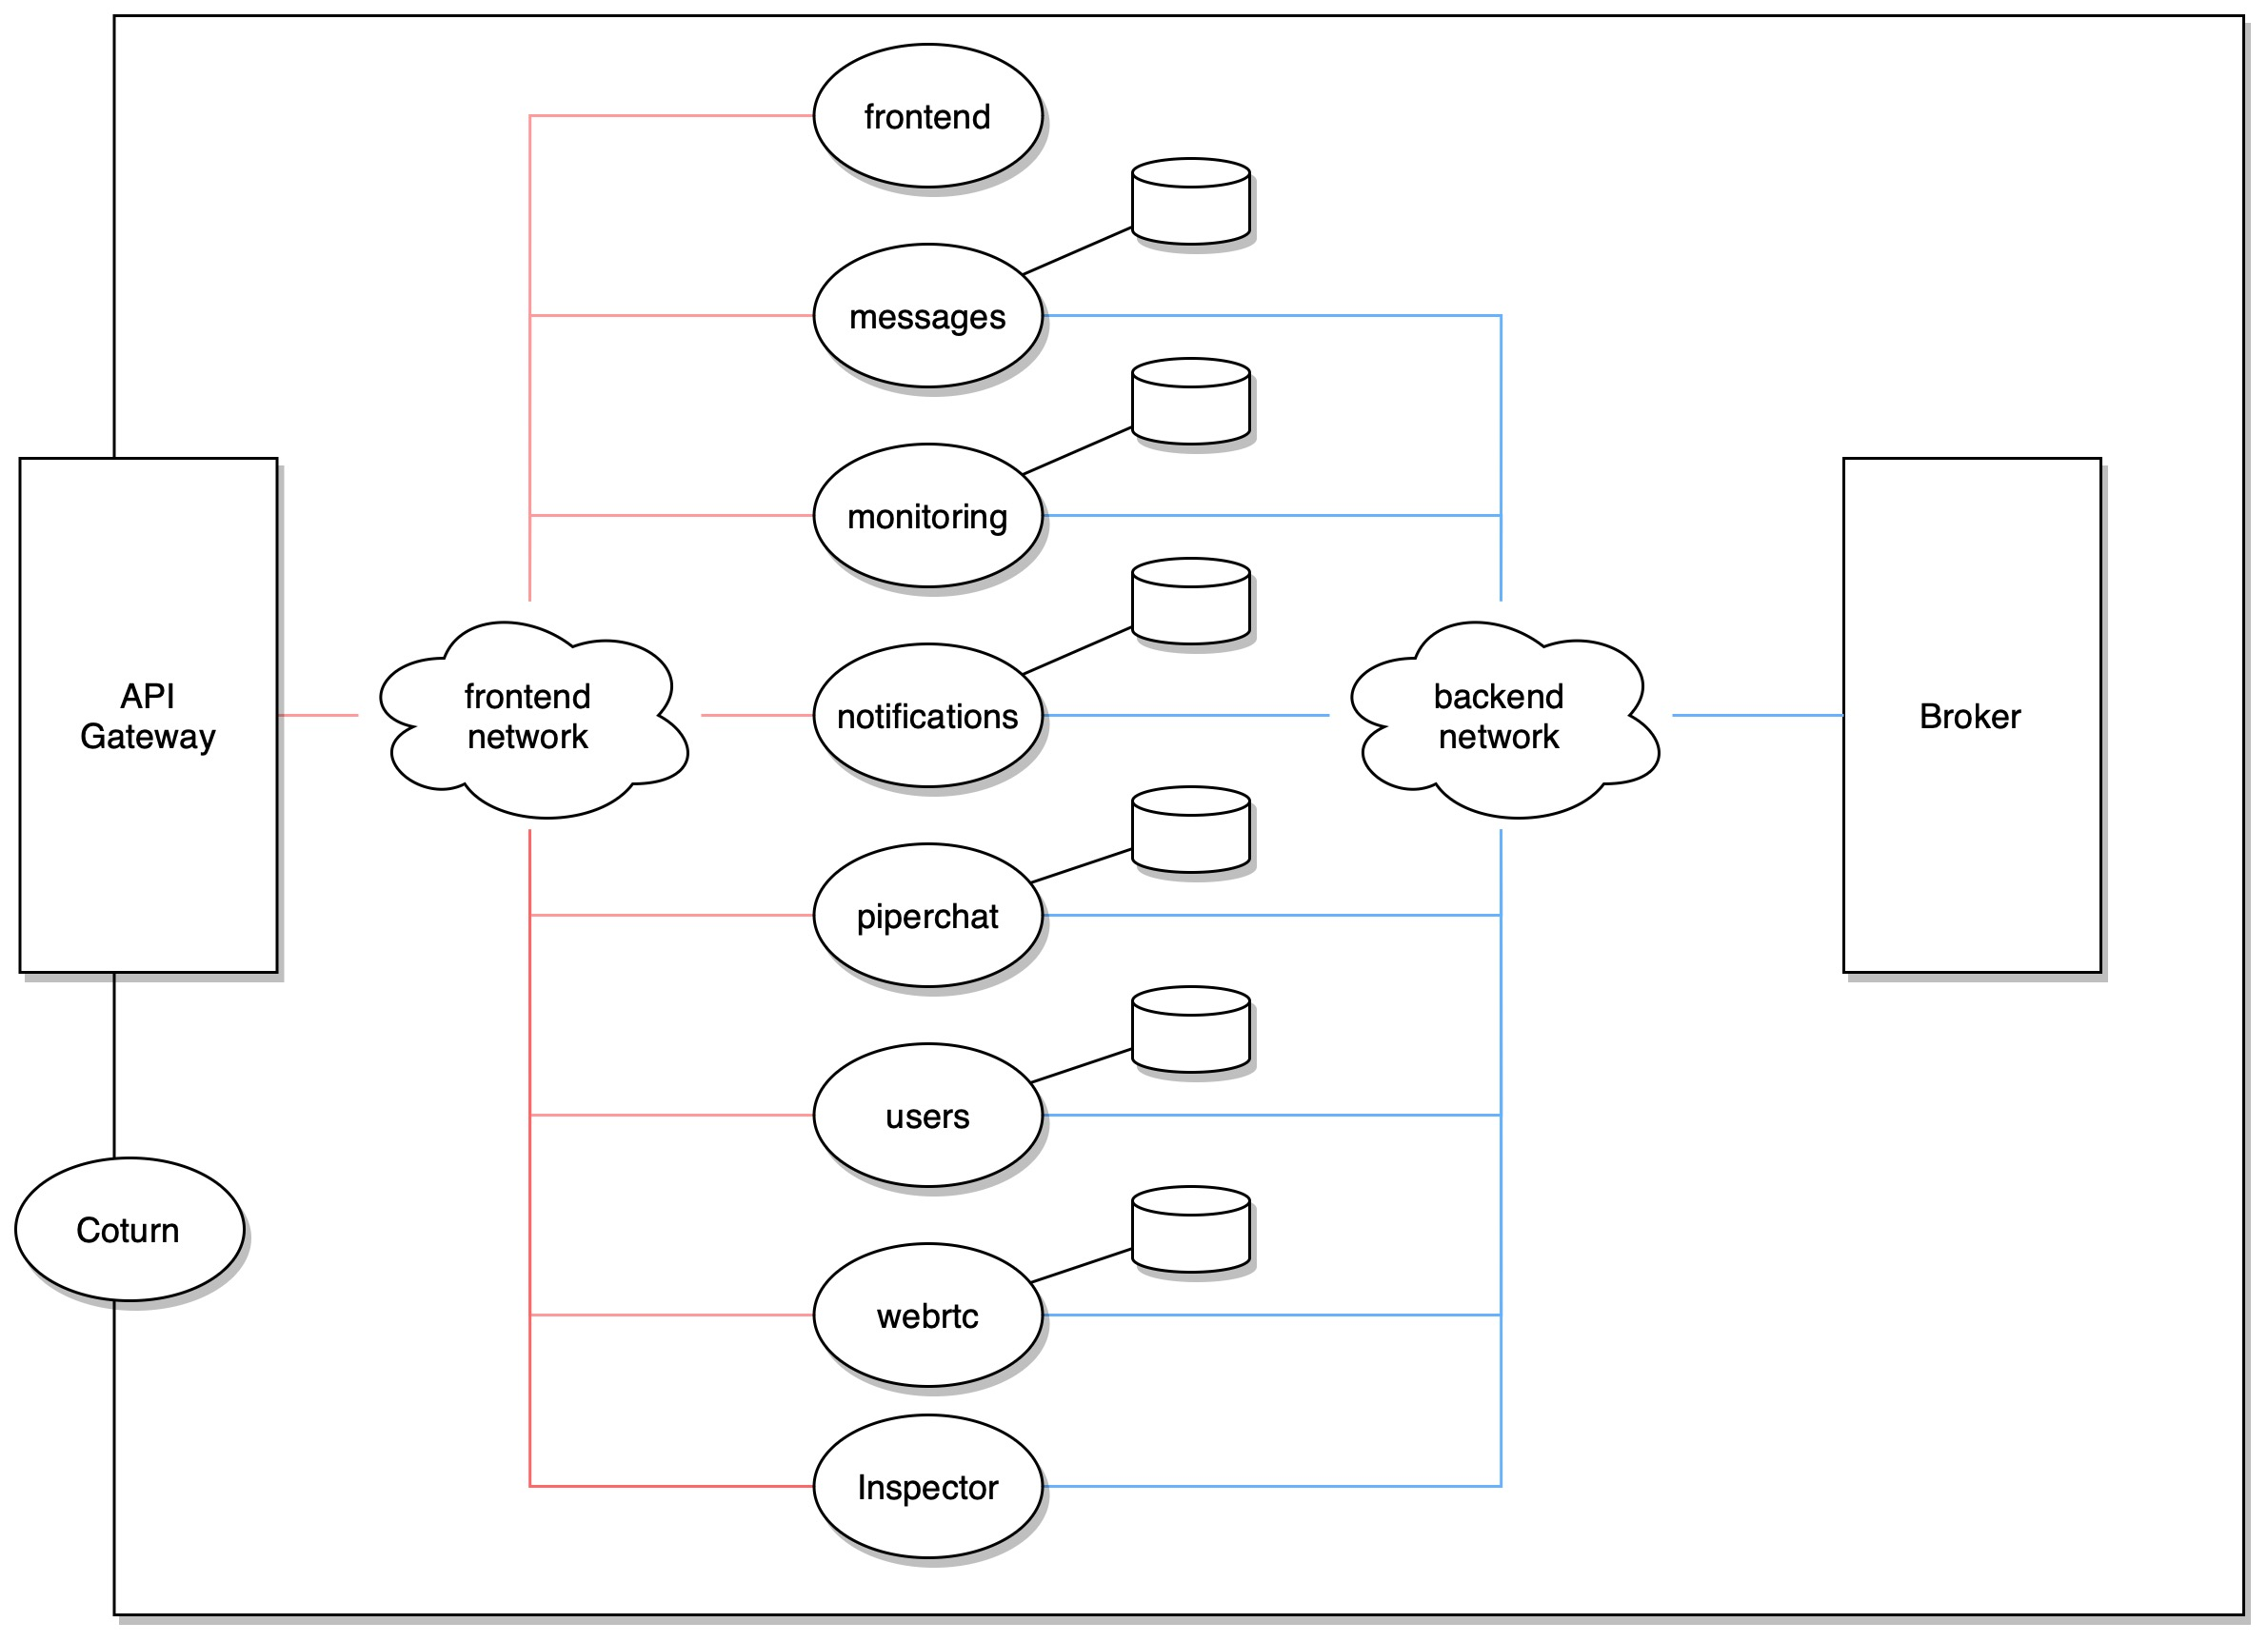
\includegraphics[width=0.85\textwidth]{img/07-deployment/architecture-deployment.jpg}
    \label{fig:architecture-deployment}
\end{figure}

%
%
%
\newpage
\section{Testing deploy}

Per effettuare il testing lato Backend, è stato realizzato un ulteriore \texttt{Docker Compose} il quale ci ha permesso deployare un infrastruttura "alleggerita", dotata unicamente dei container necessari a testare i singoli microservizi, nonché:

\begin{itemize}
    \item Un'istanza del Broker

    \item Un'istanza del database

    \item Un'istanza di Mongo Express per visualizzare il database
\end{itemize}

Questo \texttt{Docker Compose} è situato nella cartella \texttt{/dev}, insieme allo script che ne automatizza l'esecuzione, chiamato \texttt{runDev.sh}.

Di seguito riportato il \texttt{Docker Compose} dell'infrastruttura usata per il testing:

\begin{verbatim}
services:
  db-service:
    image: mongo
    ports:
      - '27017:27017'
    healthcheck:
      test: |
        host=`hostname --ip-address || echo '127.0.0.1'`;
        mongo --quiet $${host}/test --eval
            'quit(db.runCommand({ ping: 1 }).ok ? 0 : 2)' && echo 0 || echo 1

  broker:
    image: rabbitmq:3-management-alpine
    ports:
      - '5672:5672'
      - '15672:15672'
    healthcheck:
      test: ['CMD', 'rabbitmq-diagnostics', '-q', 'ping']

  mongo-express:
    image: mongo-express:latest
    restart: always
    ports:
      - '8081:8081'
    environment:
      ME_CONFIG_MONGODB_SERVER: 'db-service'
    depends_on:
      db-service:
        condition: service_healthy

\end{verbatim}
